\documentclass{article}
\usepackage{graphicx}
\usepackage{hyperref}
\usepackage{float}
\font\myfont=cmr12 at 40pt
\title{\vspace{-2cm}\myfont Gradescope Manual}
\date{\vspace{-5ex}}
\setlength\parindent{24pt}

\begin{document}
  \maketitle

\section{Part 1: Login and Access to Assignments}
\hspace{\parindent}The homework assignment of this class would be posted on Gradescope. You can access this website via \href{http://www.gradescope.com}{gradescope.com}. %can edit to direct to course page. 
When asked to login, use school credentials and select USCB NetID.\\*
\begin{figure}[h!]
\centerline{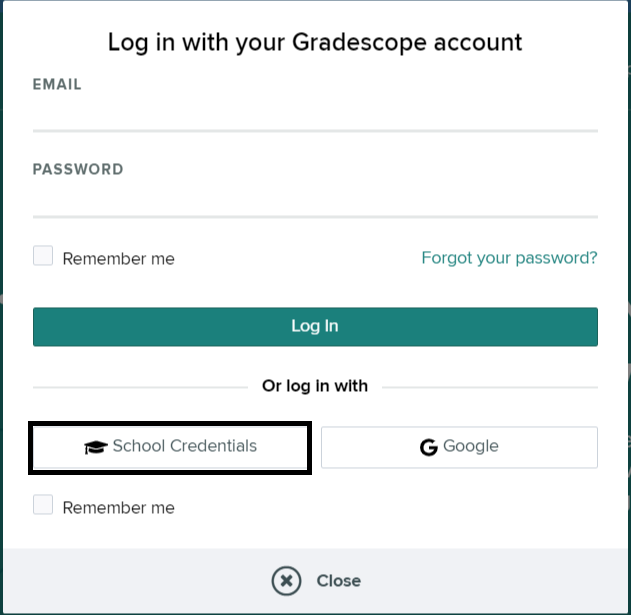
\includegraphics[scale=.5]{login_1.png}}
\caption{Choose School Credential Portal}
\label{fig}
\end{figure}
\begin{figure}[H]
\centerline{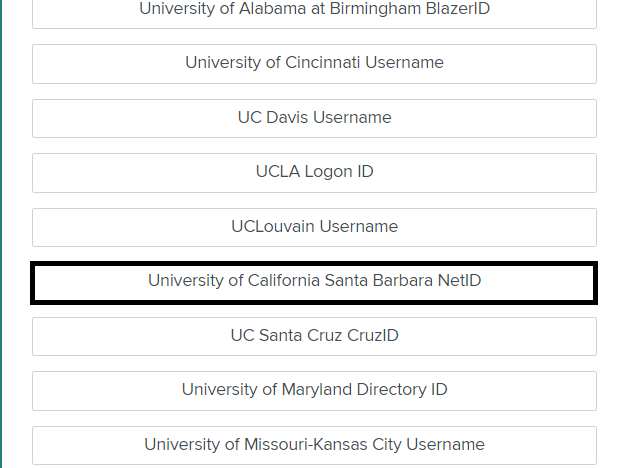
\includegraphics[scale=.5]{login_2.png}}
\caption{Login Using UCSB Credentials}
\label{fig}
\end{figure}
Once logged in, you will be directed to your workspace where you will be able to access all courses which use gradescope.
Find Econ 145 by selecting the respective tab. From this page, you may view the assignments, their respective due dates and submission status. 
\section{Part 2: Submitting Homeworks}
\hspace{\parindent}The course panel displays information regarding each assignments. You would be able to view your highest submission score, due dates and late due dates if applicable. \\*
\begin{figure}[h]
\centerline{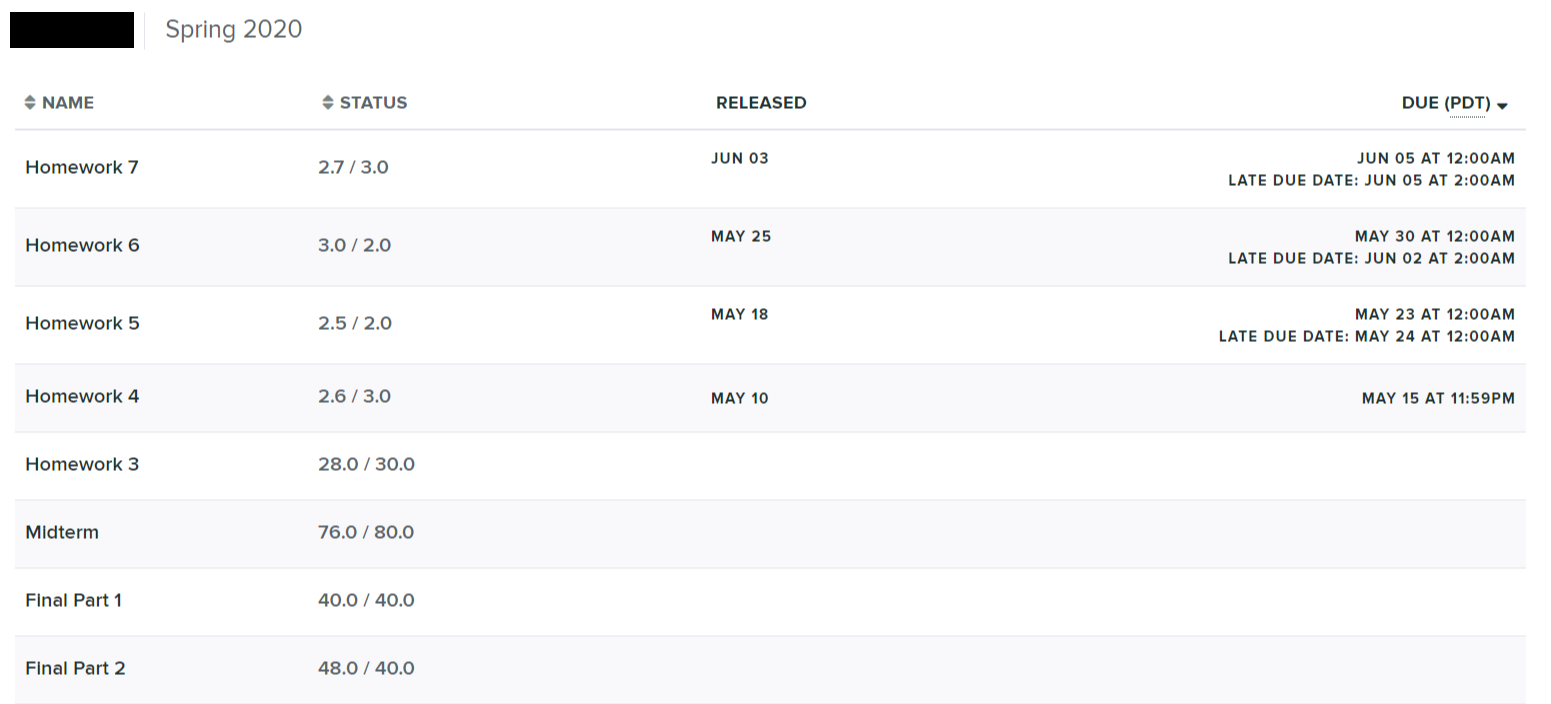
\includegraphics[scale=.5]{Assignment.png}}
\label{fig}
\end{figure}

In Econ 145, you should expect two types of assignments. Coding and write-up assignnments. The general uploading procedure for both assignments are similar. 
\subsection{Write-up submission}
\hspace{\parindent}To submit, click on the respective assignment, and choose upload PDF.
\begin{figure}[H]
\centerline{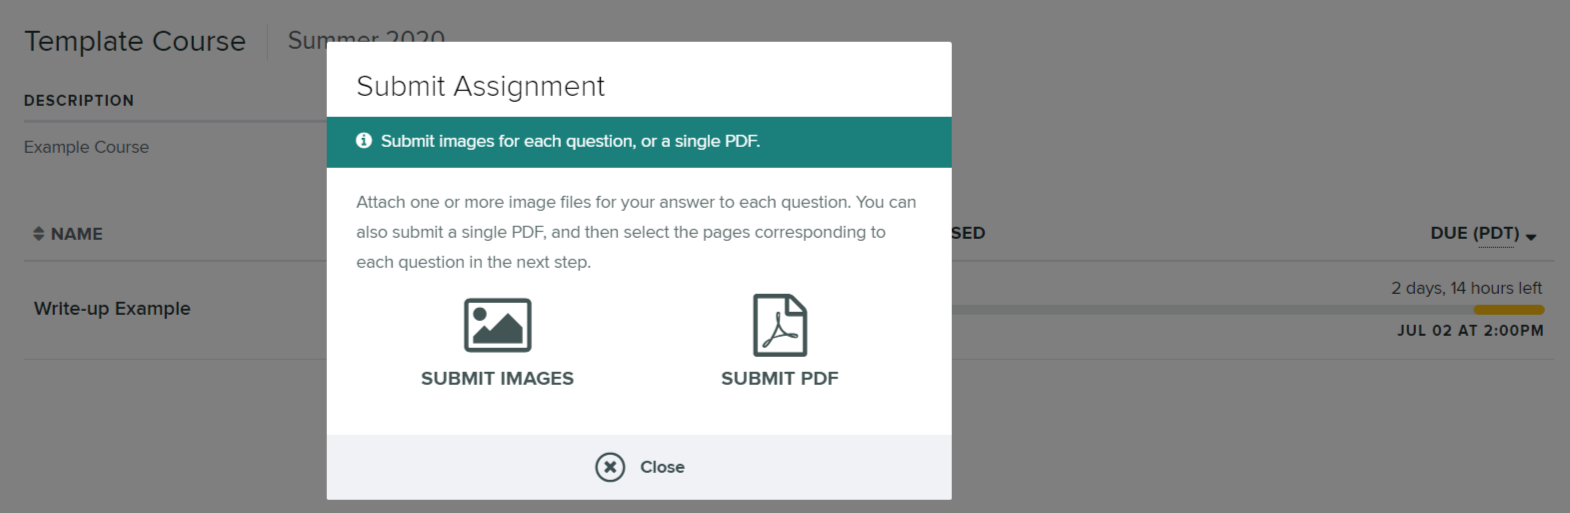
\includegraphics[scale=.25]{submit_1.png}}
\label{fig}
\end{figure}
After submitting files, please proceed to mark Questions with correct page(s). And click on submit. 
\begin{figure}[H]
\centerline{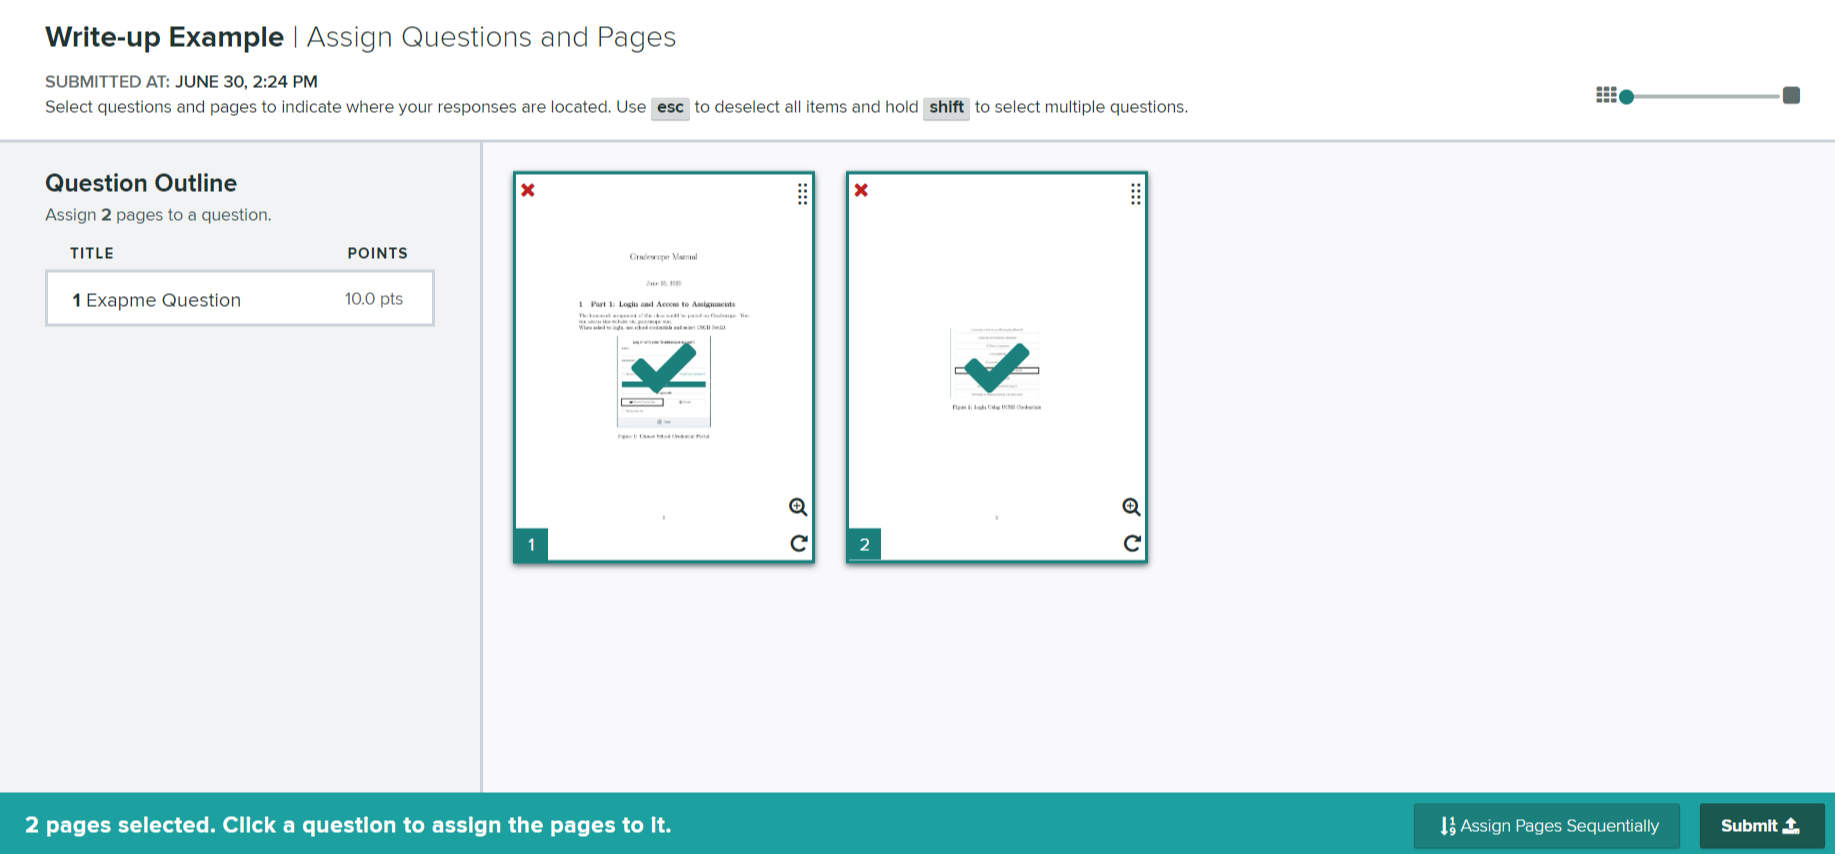
\includegraphics[scale=.25]{submit_2.png}}
\caption{Please mark each page with correct questions}
\label{fig}
\end{figure}
Once a submission is made, you should be able to view your submission, reselect pages and resubmit files until deadline is passed.
\subsection{Coding submission}
\hspace{\parindent}Go to the Course tab, and select the coding assignment you wish to submit.
Choose to upload from local files, and make sure to name your files correctly. CAPITALS do matter.
\begin{figure}[H]
\centerline{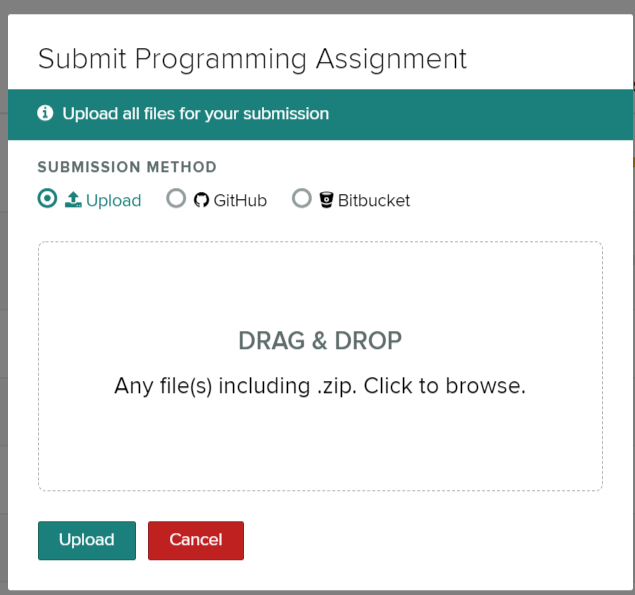
\includegraphics[scale=.5]{submit_3.png}}
\caption{Please choose the first upload option as the latter could cause unwanted problems}
\label{fig}
\end{figure}
The coding assignments use autograders that could provide result and feedbacks automatically.
You should be able to revisit and review comments for each questions until the deadline.
If you wish to change anything, use resubmit function.
\subsection{}
To sum, the steps to upload homeworks are:\\*
1: Go to respective homework tab;\\*
2: Click on Submit, and choose correct files to upload;\\*
3: For coding assignments, make sure the files are properly named, CAPITALS do matter;\\*
4: For write-up assignments, assign each questions correctly;\\*
5: Click upload, you should get email notification if submission is successful;\\*
6: Revisit and resubmit homework if necessary.
\section{Part 3: Regrade}
\hspace{\parindent}Gradescope allowed for regrade request after the deadline is passed and scores are published. (Note that regrade requests are not always enabled and are avaiblable at instructors' discretion.) To regrade, go to the assignments that you wish to regrade, and choose the question(s) to submit regrade request. 
\begin{figure}[H]
\centerline{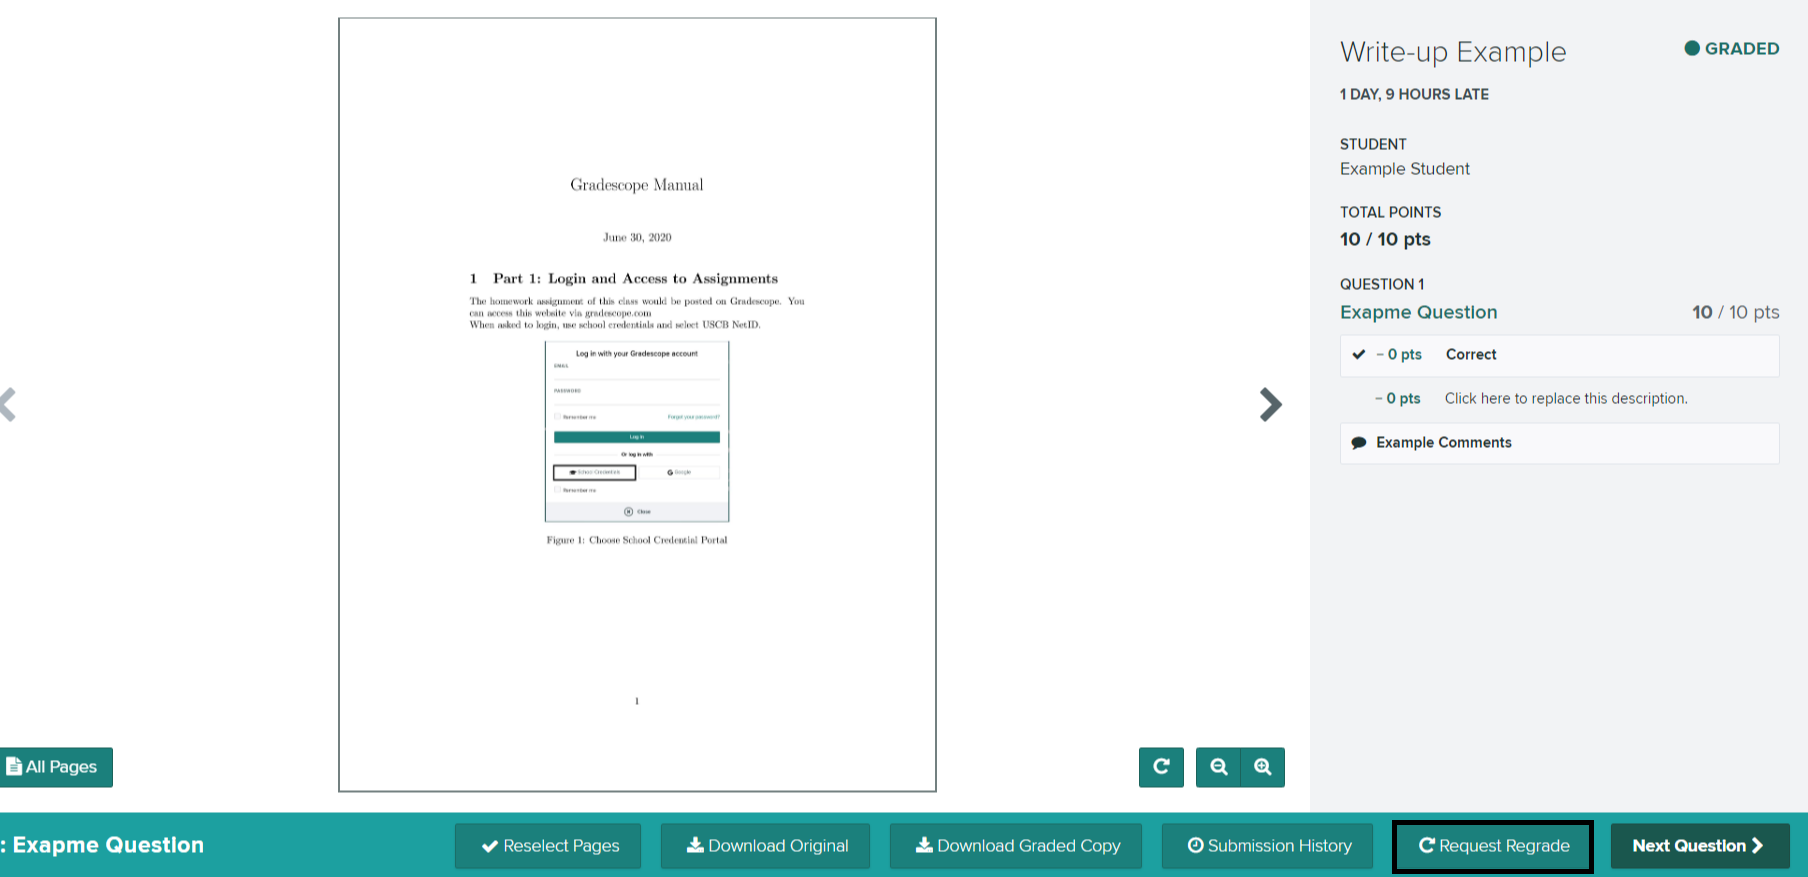
\includegraphics[scale=.5]{regrade.png}}
\label{fig}
\end{figure}
Gradescope operates on a per-question basis. Please submit requests for each respective question you wish to regrade.
\end{document}